\chapter{Methodology and Results}

THE TEXTHEIGHT IS \the\textheight
THE TEXt width IS \the\textwidth

The previous section outlined the procedure for using Bayesian inference to solve a simple regression problem. It then expanded the concept to allowing for regression where the data is not in the same space as the inference result. The two spaces being connected by a forward model or responce matrix. This is exactly what is required as interferometry data is not in the same space as the profile to be inferred. Two main methods for dealing with the hyperparameters were also outlined. They are \gls{map} and marginalisation. Results will be presented for both sections. Both allow for hyperpriors to be included. A uniform prior is used for all hyperparameters and the bounds were selected by carefully observing how the parameters affect the resulting inferrence and allowing generous amount of room for profile extreamities to exist. The amplitude is constrained between $0$ and $100$ and is on the same scale as the electron density $\cdot 10^{20}$. Each length scale is bounded between 0 and 3 and is on the same scale as the normalised radius. This includes the non static kernel varients hyperbolic tangent length scale and cubic spline length scale. 5 knots were used for the cubic spline. To reduce the dimensionality of the problem they were evenly spaced across the normalised radius. Each interferometry channel is assumed to have the same experimental error and it is bounded between $0.03$ and $0.3\, \cdot10^{-19}m^2$. WEST reports a no plasma noise in the order of $0.03 \cdot10^{-19}m^2$. The hyperparameter \gls{map} is found by minimising the loss function based on the marginal likelihood, see equation \ref{eq:loss}. When any trialed parameters exceed their prior bounds the loss returns infinity (or a very high number). SciPy minimise and PyTorch SGD are both gradient based methods that were trialed and achieved similar results. In order to precisely measure the accuracy of the inferences a known ground truth profile is required. The metric used is mean square error and is included on each graph as `mse'. There are a few main profile types of interest to the scientific community. L mode or low confinement profiles are typically parabolic like in shape and are the bread an butter of tokamak operation. It is the easiest profile to achieve and is often a stepping stone to achiving other profiles within a plasma shot. This is the main profile used within the \gls{west} tokamak. H mode or high confinement mode is achieved by increasing external heating power from sources such as neutral bean injection and electron cyclotron resonance heating. H mode profiles have a distinct sharp drop in density near the plasma boundary. H mode profiles are well known for largely increasing the energy confinement time of the plasma which is a cruicial factor for net positive energy production. Although they do introduce extra instabilites known as ELMS. Another interesting profile feature is known as peaking. The external heating elements can be tuned to target the core. The extra heat ionises more of the fuel and decreases electrion-ion recombination rates. This increases the electron density in the core and creates a peak or bell shape profile. This can be achieved with both L mode and H mode. Peaking is known to increase the stability and performance of the plasma. It helps reduce the impurities in the core that contribute to radiation loss. Versions of these profiles are shown in figure \ref{fig:groundtruth}. The interferomety data that would be measured given a profile as the ground truth is computed with the responce matrix. The responce matrix is created using real magnetic field lines inffered by \gls{nice}. A generously small Gaussian experimental error is added with a standard deviation of $3\cdot10^-17 \, m^2$. This is what \gls{west} reports as the no plasma noise of the interferometer. 


\begin{figure}[ht]
    \centering
    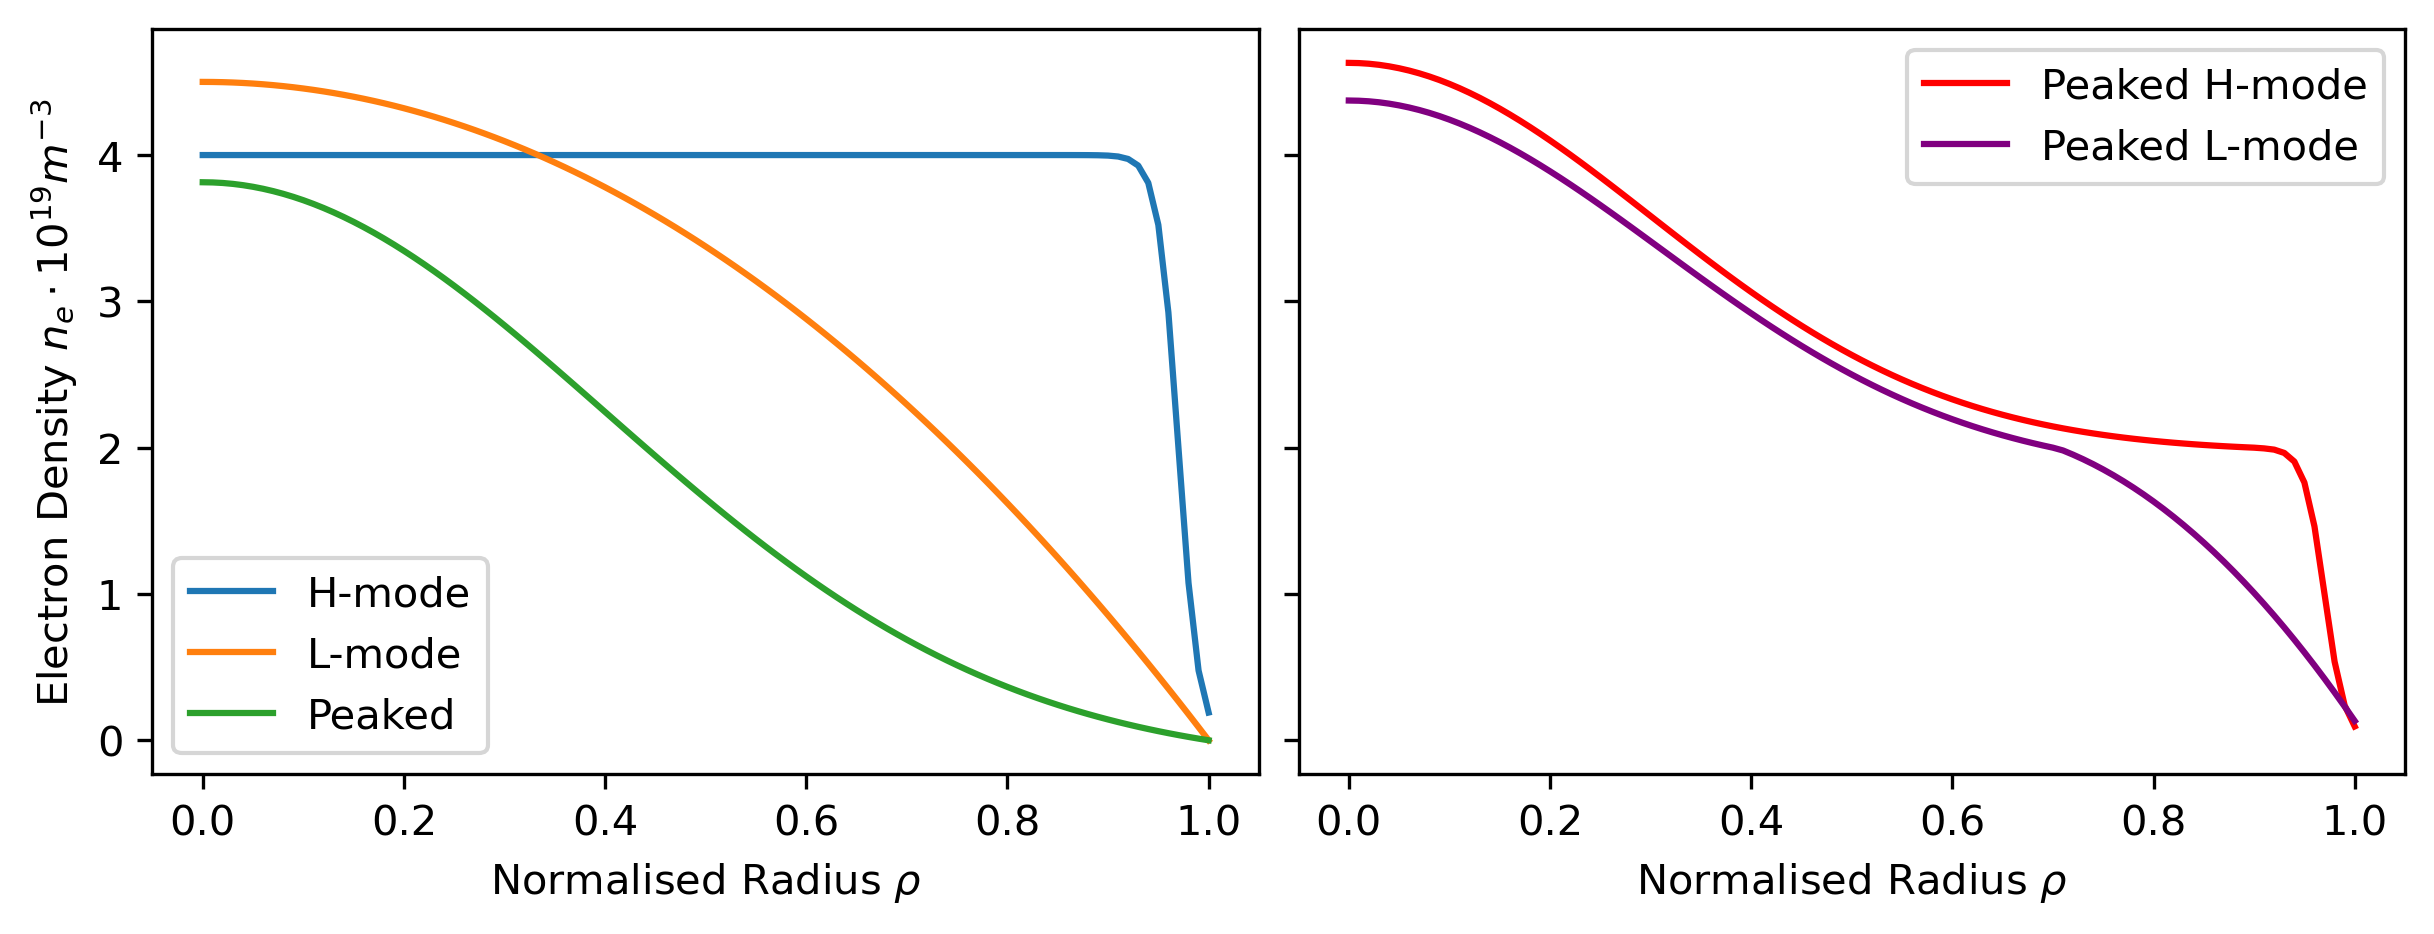
\includegraphics[width=\textwidth]{images/syntheticProfiles.png}
    \caption{Ground truth profiles used to generate synthetic interferometry data.}
    \label{fig:groundtruth}
\end{figure}

\begin{figure}[ht]
    \centering
    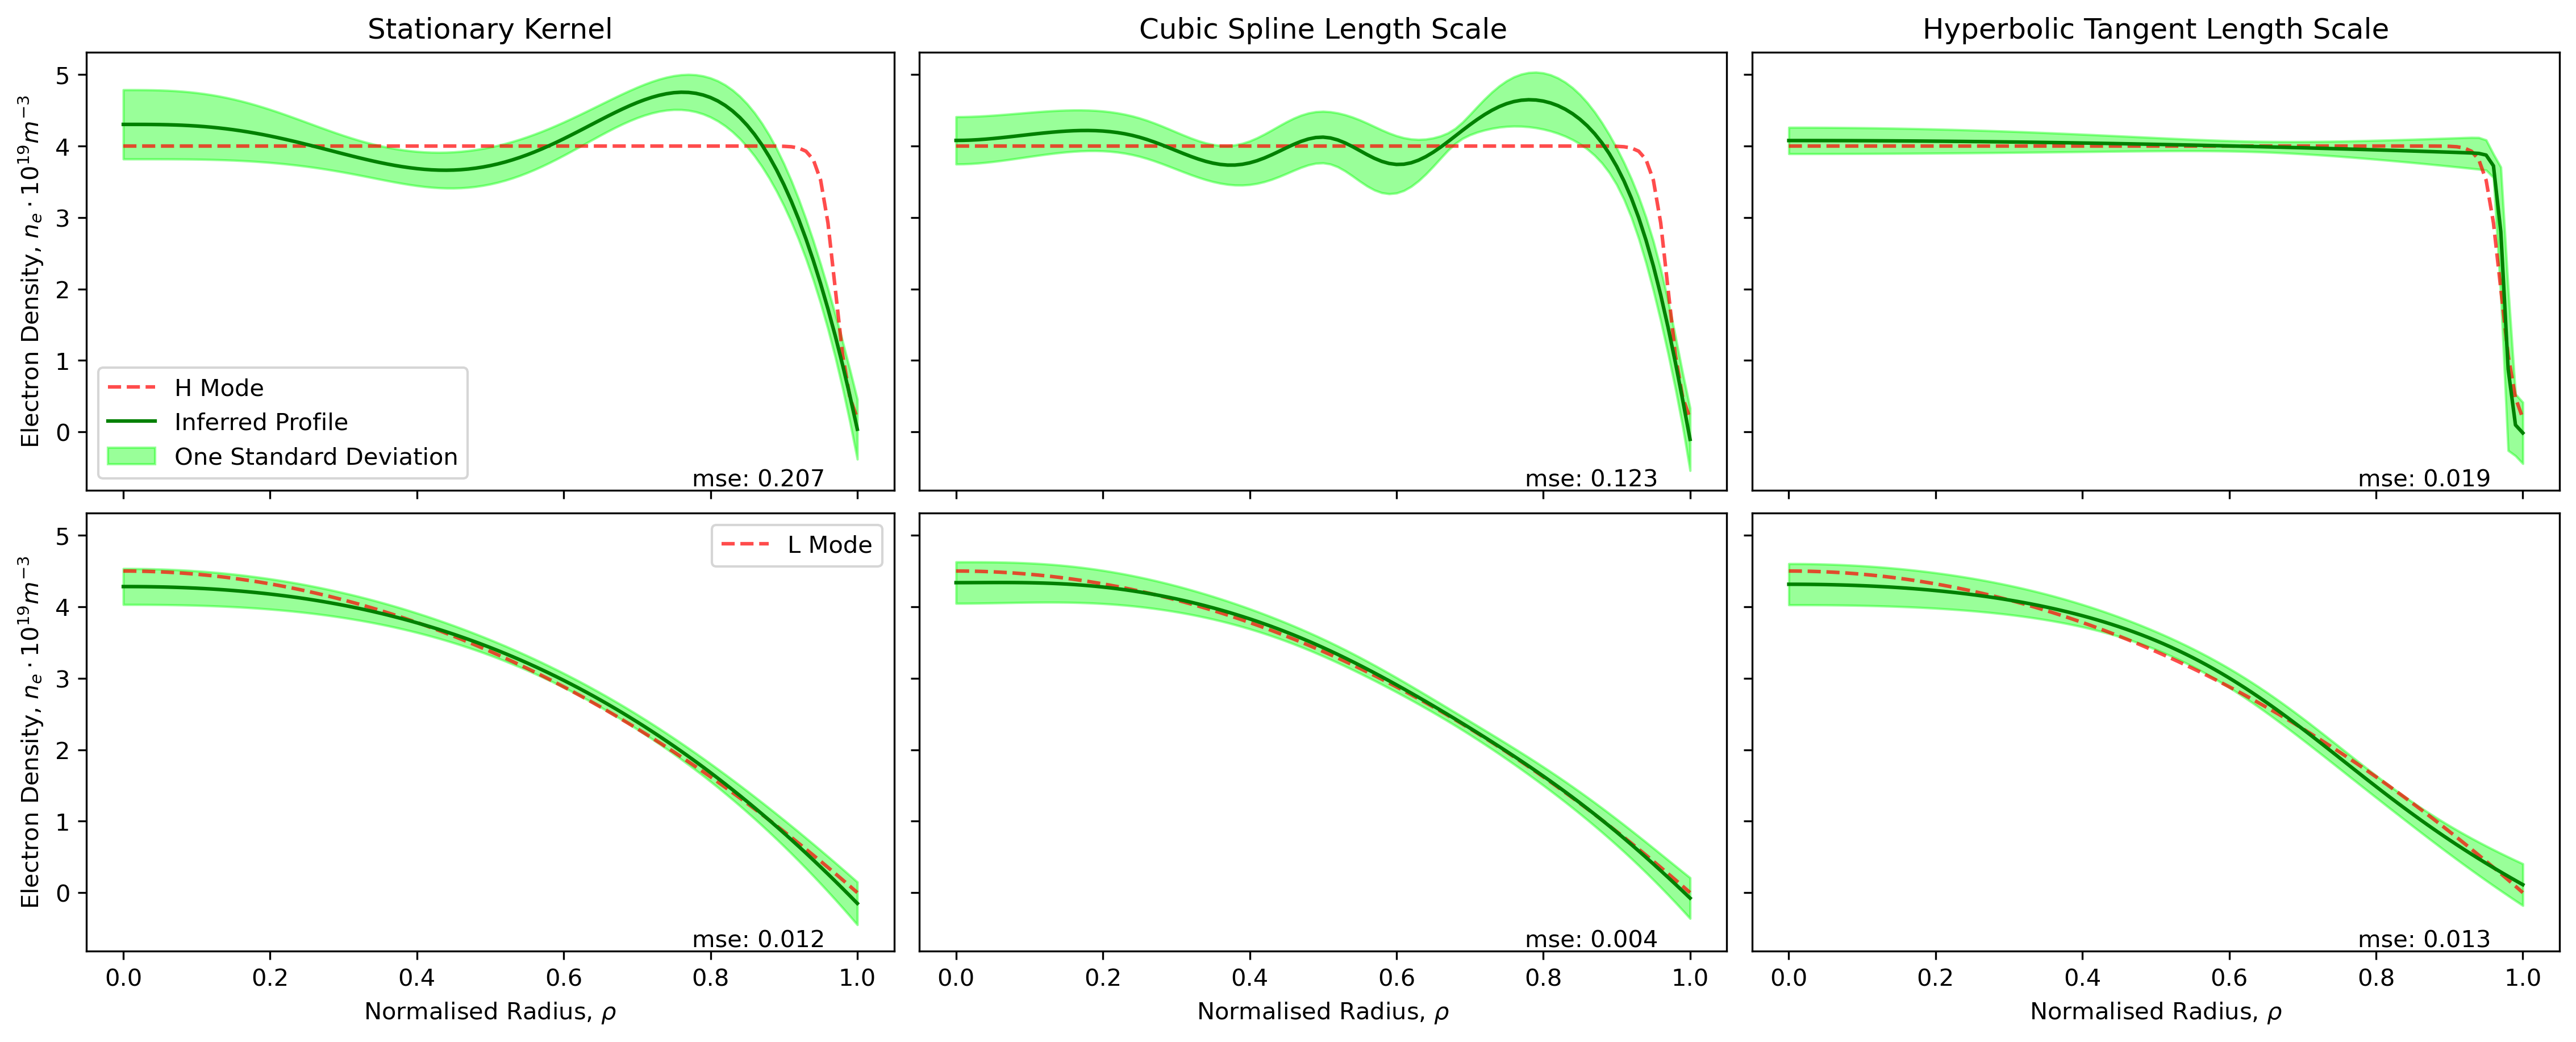
\includegraphics[width=500pt, angle=90]{images/Final/MAPsynthetic_final_hl.png}
    \caption{Electron density inference using the hyperparameter MAP method on synthetic interferometry data from H and L mode profiles.}
    \label{fig:mapsynthetic_hl}
\end{figure}

As expected the hyperbolic tangent was the most sucessfull at inferring the H mode profile, see figure \ref{fig:mapsynthetic_hl}. This is because the constant flat top requires a high length scale yet the sharp drop requires a low length scale. A low lengthscale reduces the correlation between neighbouring inferred electron densities which is required for the high gradient at the edge. It is impressive how equally accurate and precise the three kernels are at inferring the L mode profile.  

\begin{figure}[ht]
    \centering
    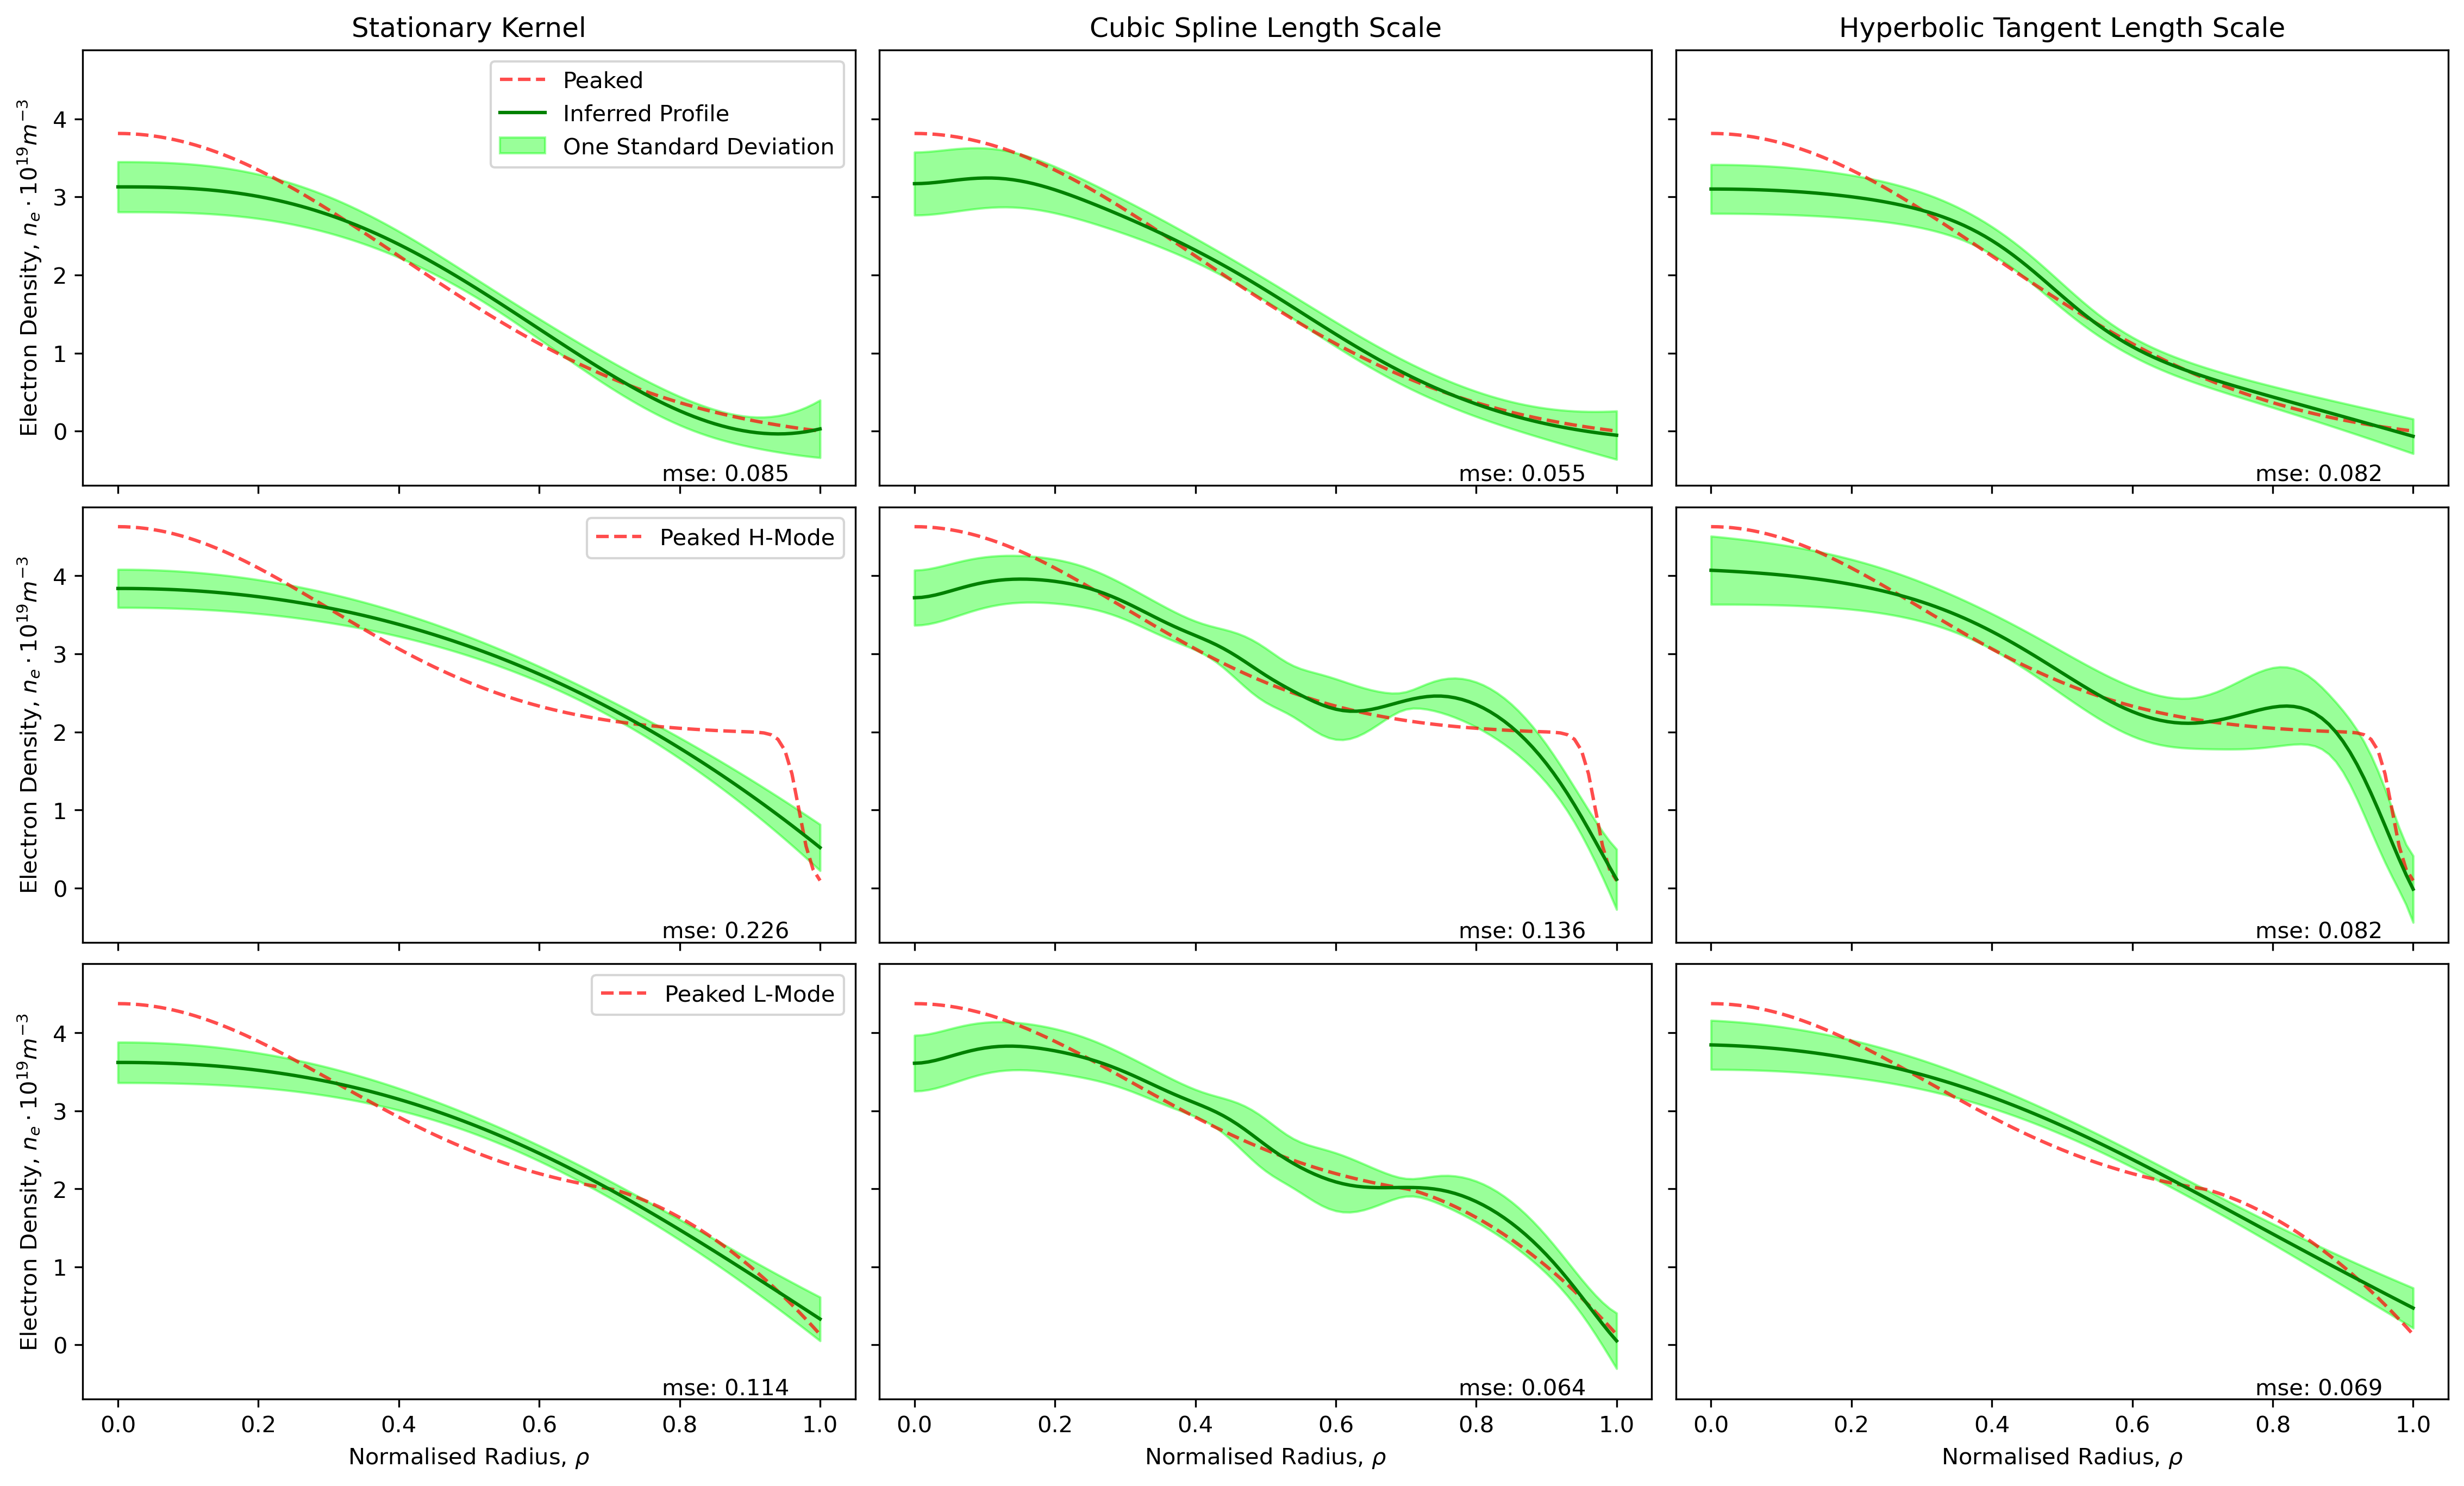
\includegraphics[width=500pt, angle=90]{images/Final/MAPsynthetic_final_p.png}
    \caption{Electron density inference using the hyperparameter MAP method on synthetic interferometry data for peaked profiles. The mean square error is shown as `mse'.}
    \label{fig:mapsynthetic_p}
\end{figure}

The static kernel performed poorly when faced with a more complex shape such as the peaked L and H mode profiles, see figure \ref{fig:mapsynthetic_p}. It appears close to parabolic and this is likely due to the length scale being inferred too large. The cubic spline length scale showcases its flexability, allowing it to find some of the profile features although this appears to come at a price of smoothness. The hyperbolic tangent was able to find the H mode edge but not as closely as it was in the pure H mode profile as the core lengthscale needed to be lower to allow for the curvy peak. It still outperformed the other kernels for the H mode peak. The hyperbolic tangent has the lowest average 'mean square error' over all the profiles at $0.053$. Cubic splines is second with $0.076$ and the stationary kernel performed the worst with $0.129$.

Marginalising the hyperparameters is an alternative approach that was introduced. This involves using \gls{mcmc} to sample from the hyperparameter posterior. This thesis uses the emcee python package which is based on the affine-invariant ensemble sampler proposed by Goodman and Weare \cite{emceeGoodman}. This method uses many `walkers' that explore the parameter space in parallel, and update their positions by placing the position of another walker into the proposal function. The advantage of this method is that it is invariant to affine transformations of the parameter space. Since a unique posterior distribution can be analytically computed from the hyperparameters, sampling hyperparameters is equilivant to sampling many posterior distributions. Since each posterior is a multivariate Gaussian sampling from them is trivial and this thesis uses the scipy stats multivariate Gaussian random variable sampler to perform the operation. One $\vec n_e$ sample is taken from each distribution. Overall this is equivalent to sampling from a posterior that is independent of the hyperparameters $P(\vec n_e | \vec d)$. To perform the \gls{mcmc} sampling the analytical expression for the predictive log marginal likelihood is used. The same prior bounds are enforced as in the \gls{map} method. 

To minimise autocorelation the emcee hyperparameters are tuned. For emcee the main hyperparameter is called `moves', which is their term for the proposal function. It is also possible to pass multiple moves and weights when sampling. Emcee will then randomly select a move in proportion to the weights. In theory, this should make the next sample more random and less correlated to the previous. Each move also has a single parameter. These can be trialled with smaller sample numbers in an attempt to minimise the autocorrelation. Optuna is a hyperparameter tuning framework for Python that proposes trials in an attempt to minimise the objective function. By default, it uses the tree-structured Parzen estimator algorithm which is also a Bayesian method. In this thesis four of the moves and their parameters are trialled with Optuna. Each trial was allowed to take 500 samples and 100 trials were made for the stationary kernel. The autocorrelation for each chain on each parameter is averaged. The lowest average autocorrelation time for each move is used to determine the parameter value of each move. It also determines the weights, allowing for the best performing move to be used more frequently. The computed weights are shown in figure \ref{fig:optuna} and this is also a probability distribution for their use when sampling.

\begin{figure}[ht]
    \centering
    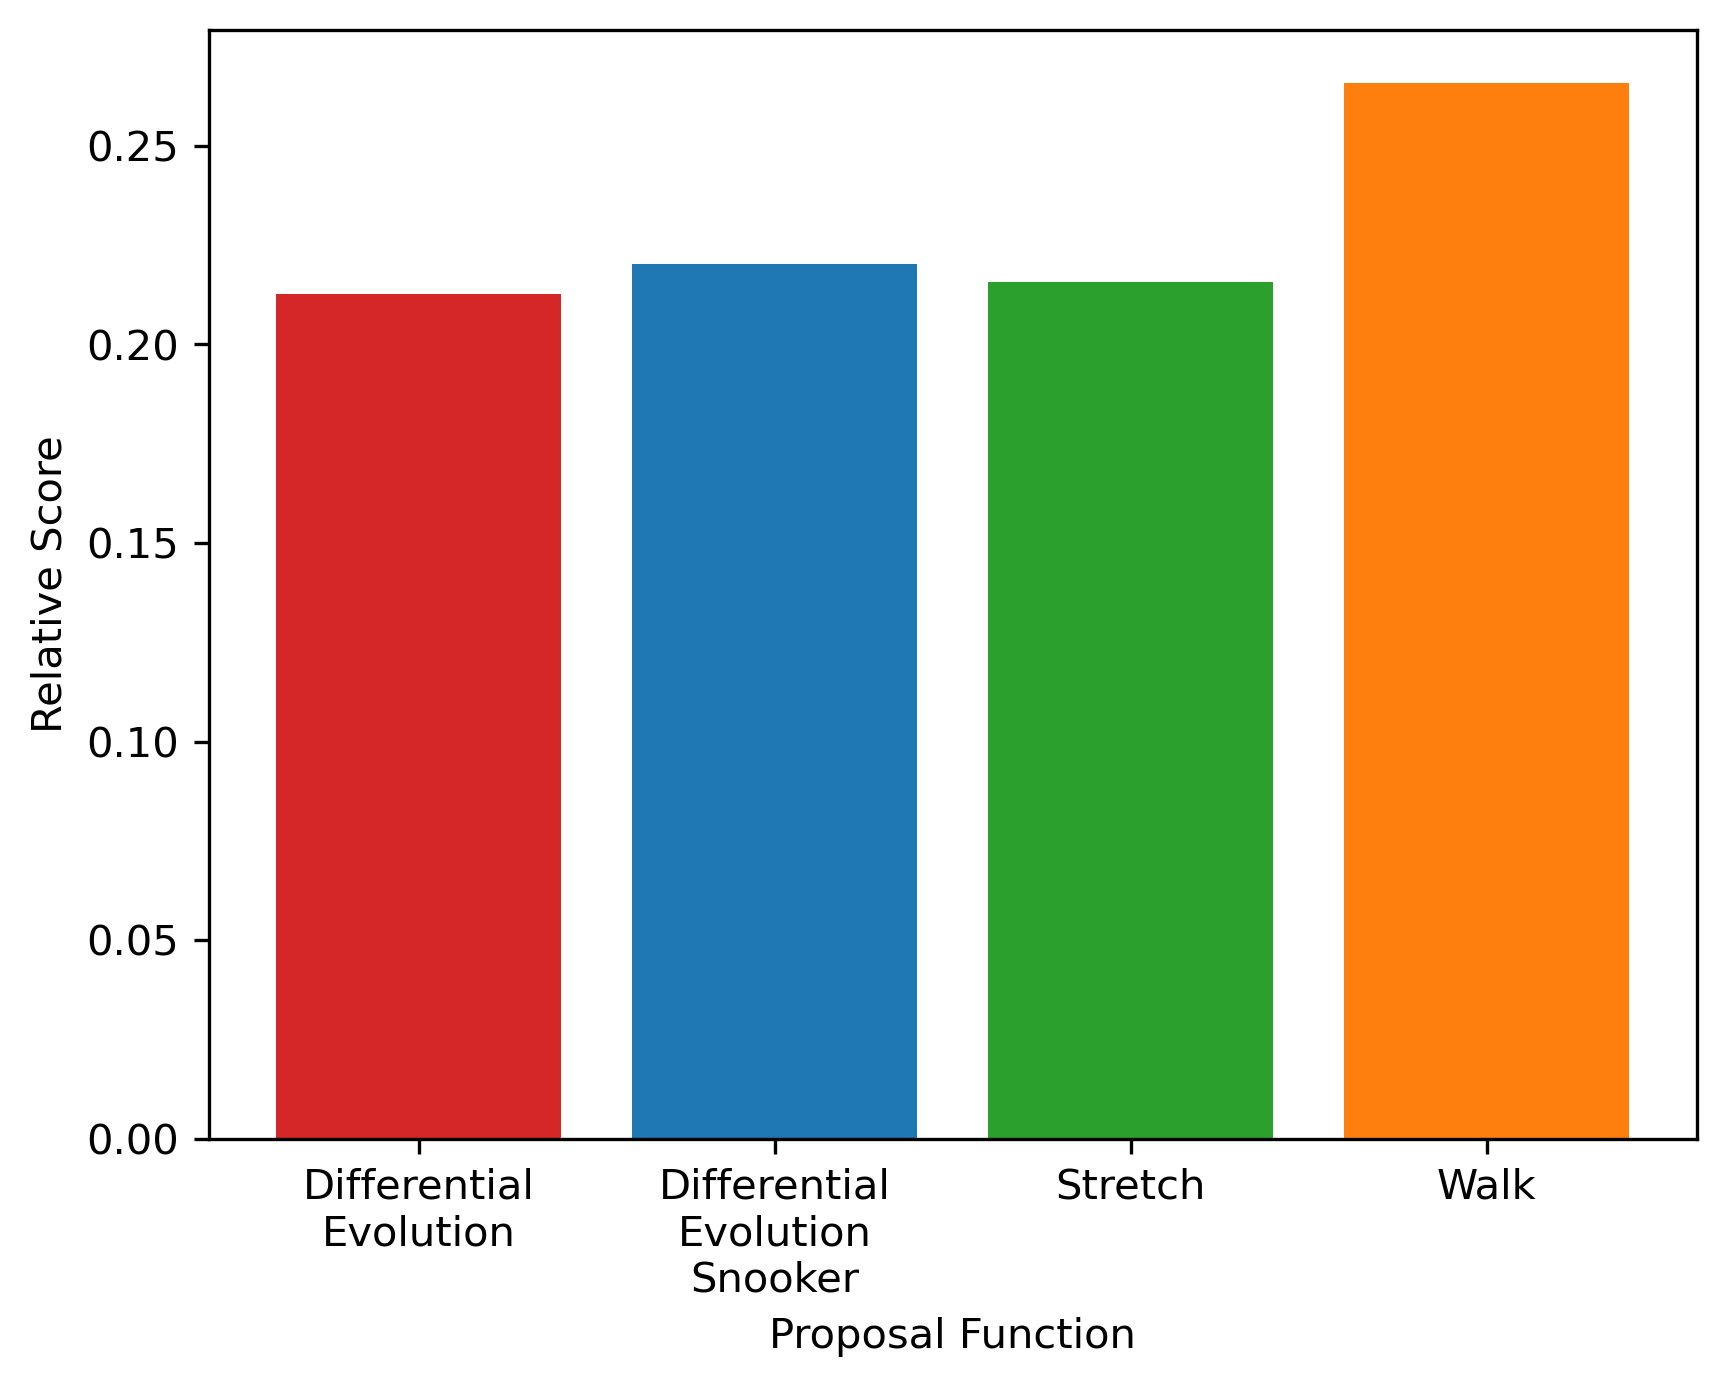
\includegraphics[width=300pt]{images/Final/optuna.png}
    \caption{The distrubution from which emcee proposal functions (moves) are selected based on perfomance in an Optuna evaluation.}
    \label{fig:optuna}
\end{figure}

They performed similarly well. Using the tuned moves combined with a burn in period of 1000 and thinning by degree 10 the autocorrlation was computed to be 23,6 for an example chain shown in figure \ref{fig:tracethin}. There still apears to be a significant amount of autocorrelation and this could affect the reliability of the results.  

\begin{figure}[ht]
    \centering
    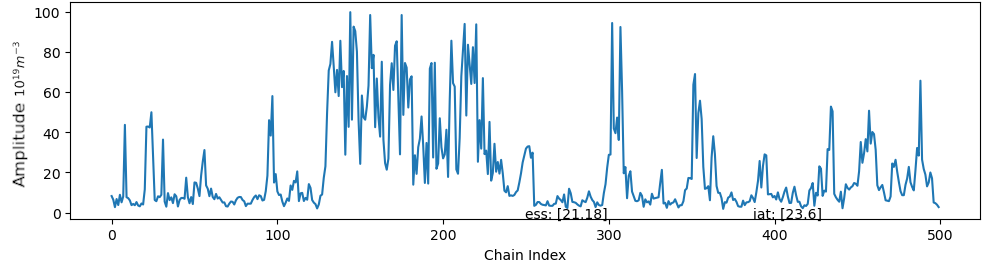
\includegraphics[width=\textwidth]{images/Final/TraceBurn1000_thin10.png}
    \caption{A trace plot showing the amplitude samples left after a burn of 1000 and thin of degree 10. The integrated autocorrelation time and effective sample size is shown as `iat' and `ess', respectivly.}
    \label{fig:tracethin}
\end{figure}

Tuning the emcee moves was not repeated for each kernel to save on computation. The same move weights are used to sample hyper parameters for the hyperbolic tangent and cubic spline non stationary kernels. 6000 samples with a burn of 1000 and thining of 10 is also used for these. The remaining 500 samples is used to compute 500 fixed parameter posteriors. One $\vec n_e$ is sampled per posterior with SciPy stats. Finally a mean and standard deviation is taken of these 500 $\vec n_e$ samples to obtain the final inferrence and uncertianty, see figures \ref{fig:fb_inference_hl} and \ref{fig:fb_inference_p}. Taking the mean and standard deviation allows for an easier comparison to the \gls{map} results. The distribution of $n_e$ at a point of normalised radius is plotted to ensure the mean is a suitable average to use, see figure \ref{fig:ne_dist}. The median and quantiles are also acceptable measures.

\begin{figure}[ht]
    \centering
    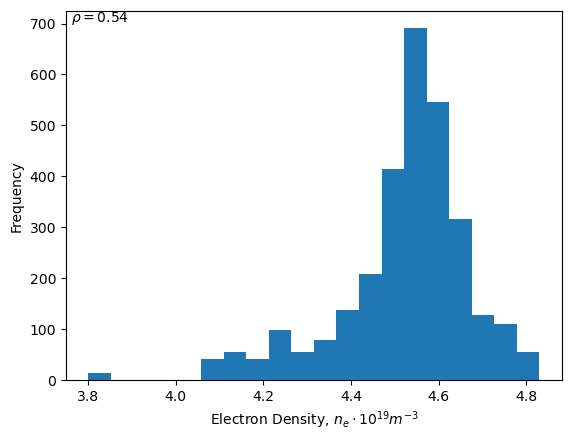
\includegraphics[width=300pt]{images/Final/sampled_ne_dist.png}
    \caption{An example distribution of $n_e$ for $\rho=0.54$ from the full Bayesian sampling method.}
    \label{fig:ne_dist}
\end{figure}

\begin{figure}[ht]
    \centering
    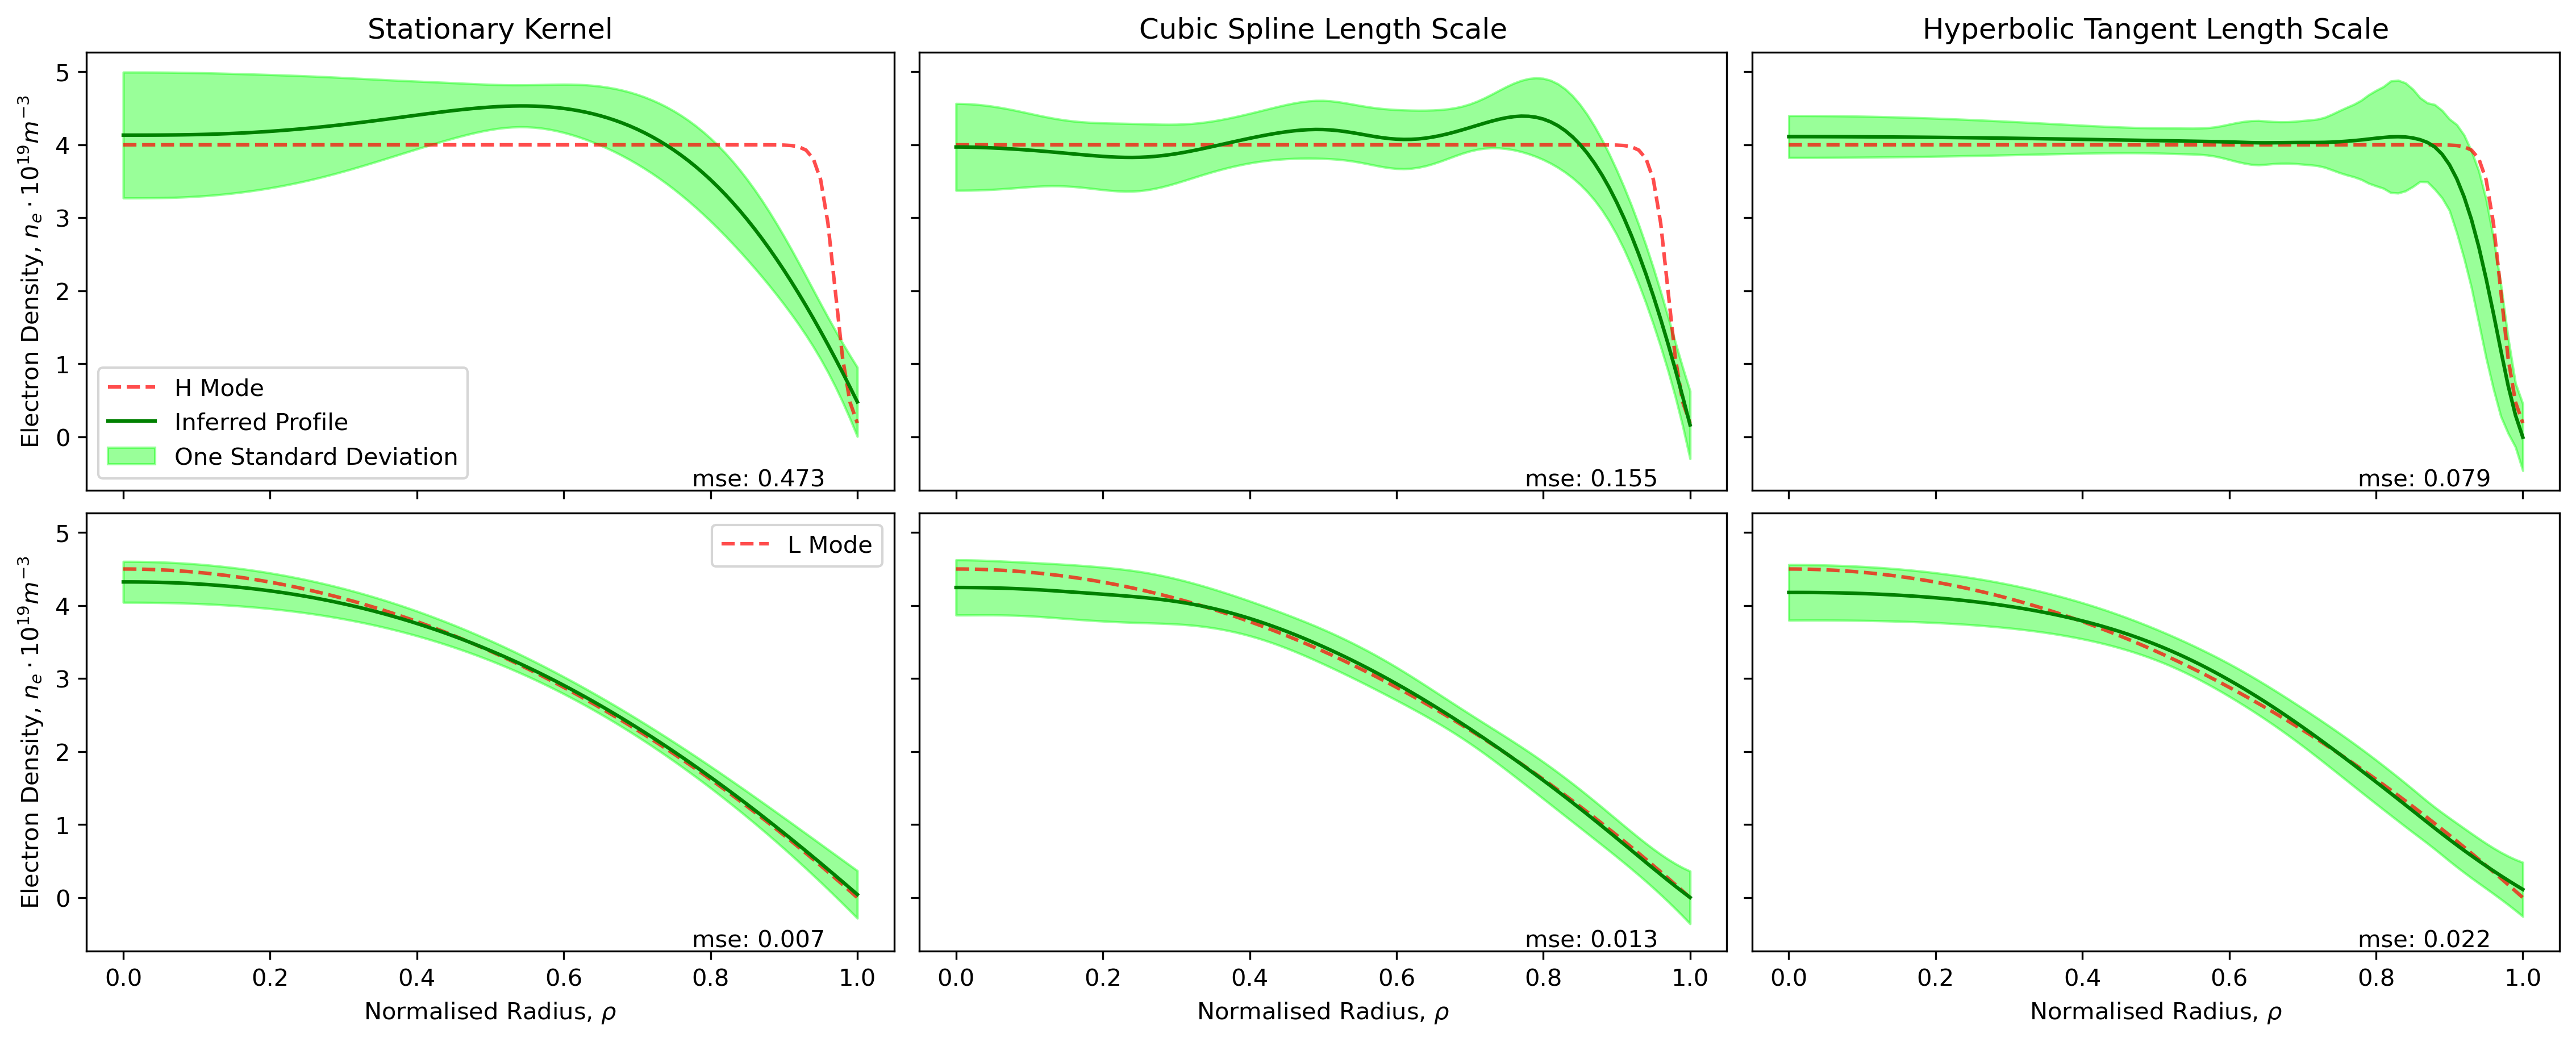
\includegraphics[width=500pt, angle=90]{images/Final/FB6000compute_noMAP_hl_burn1000_thin10.png}
    \caption{Electron density inference based on the full Bayesian method for synthetic interferometry data from H and L mode profiles. The mean square error is shown as `mse'.}
    \label{fig:fb_inference_hl}
\end{figure}


\begin{figure}[ht]
    \centering
    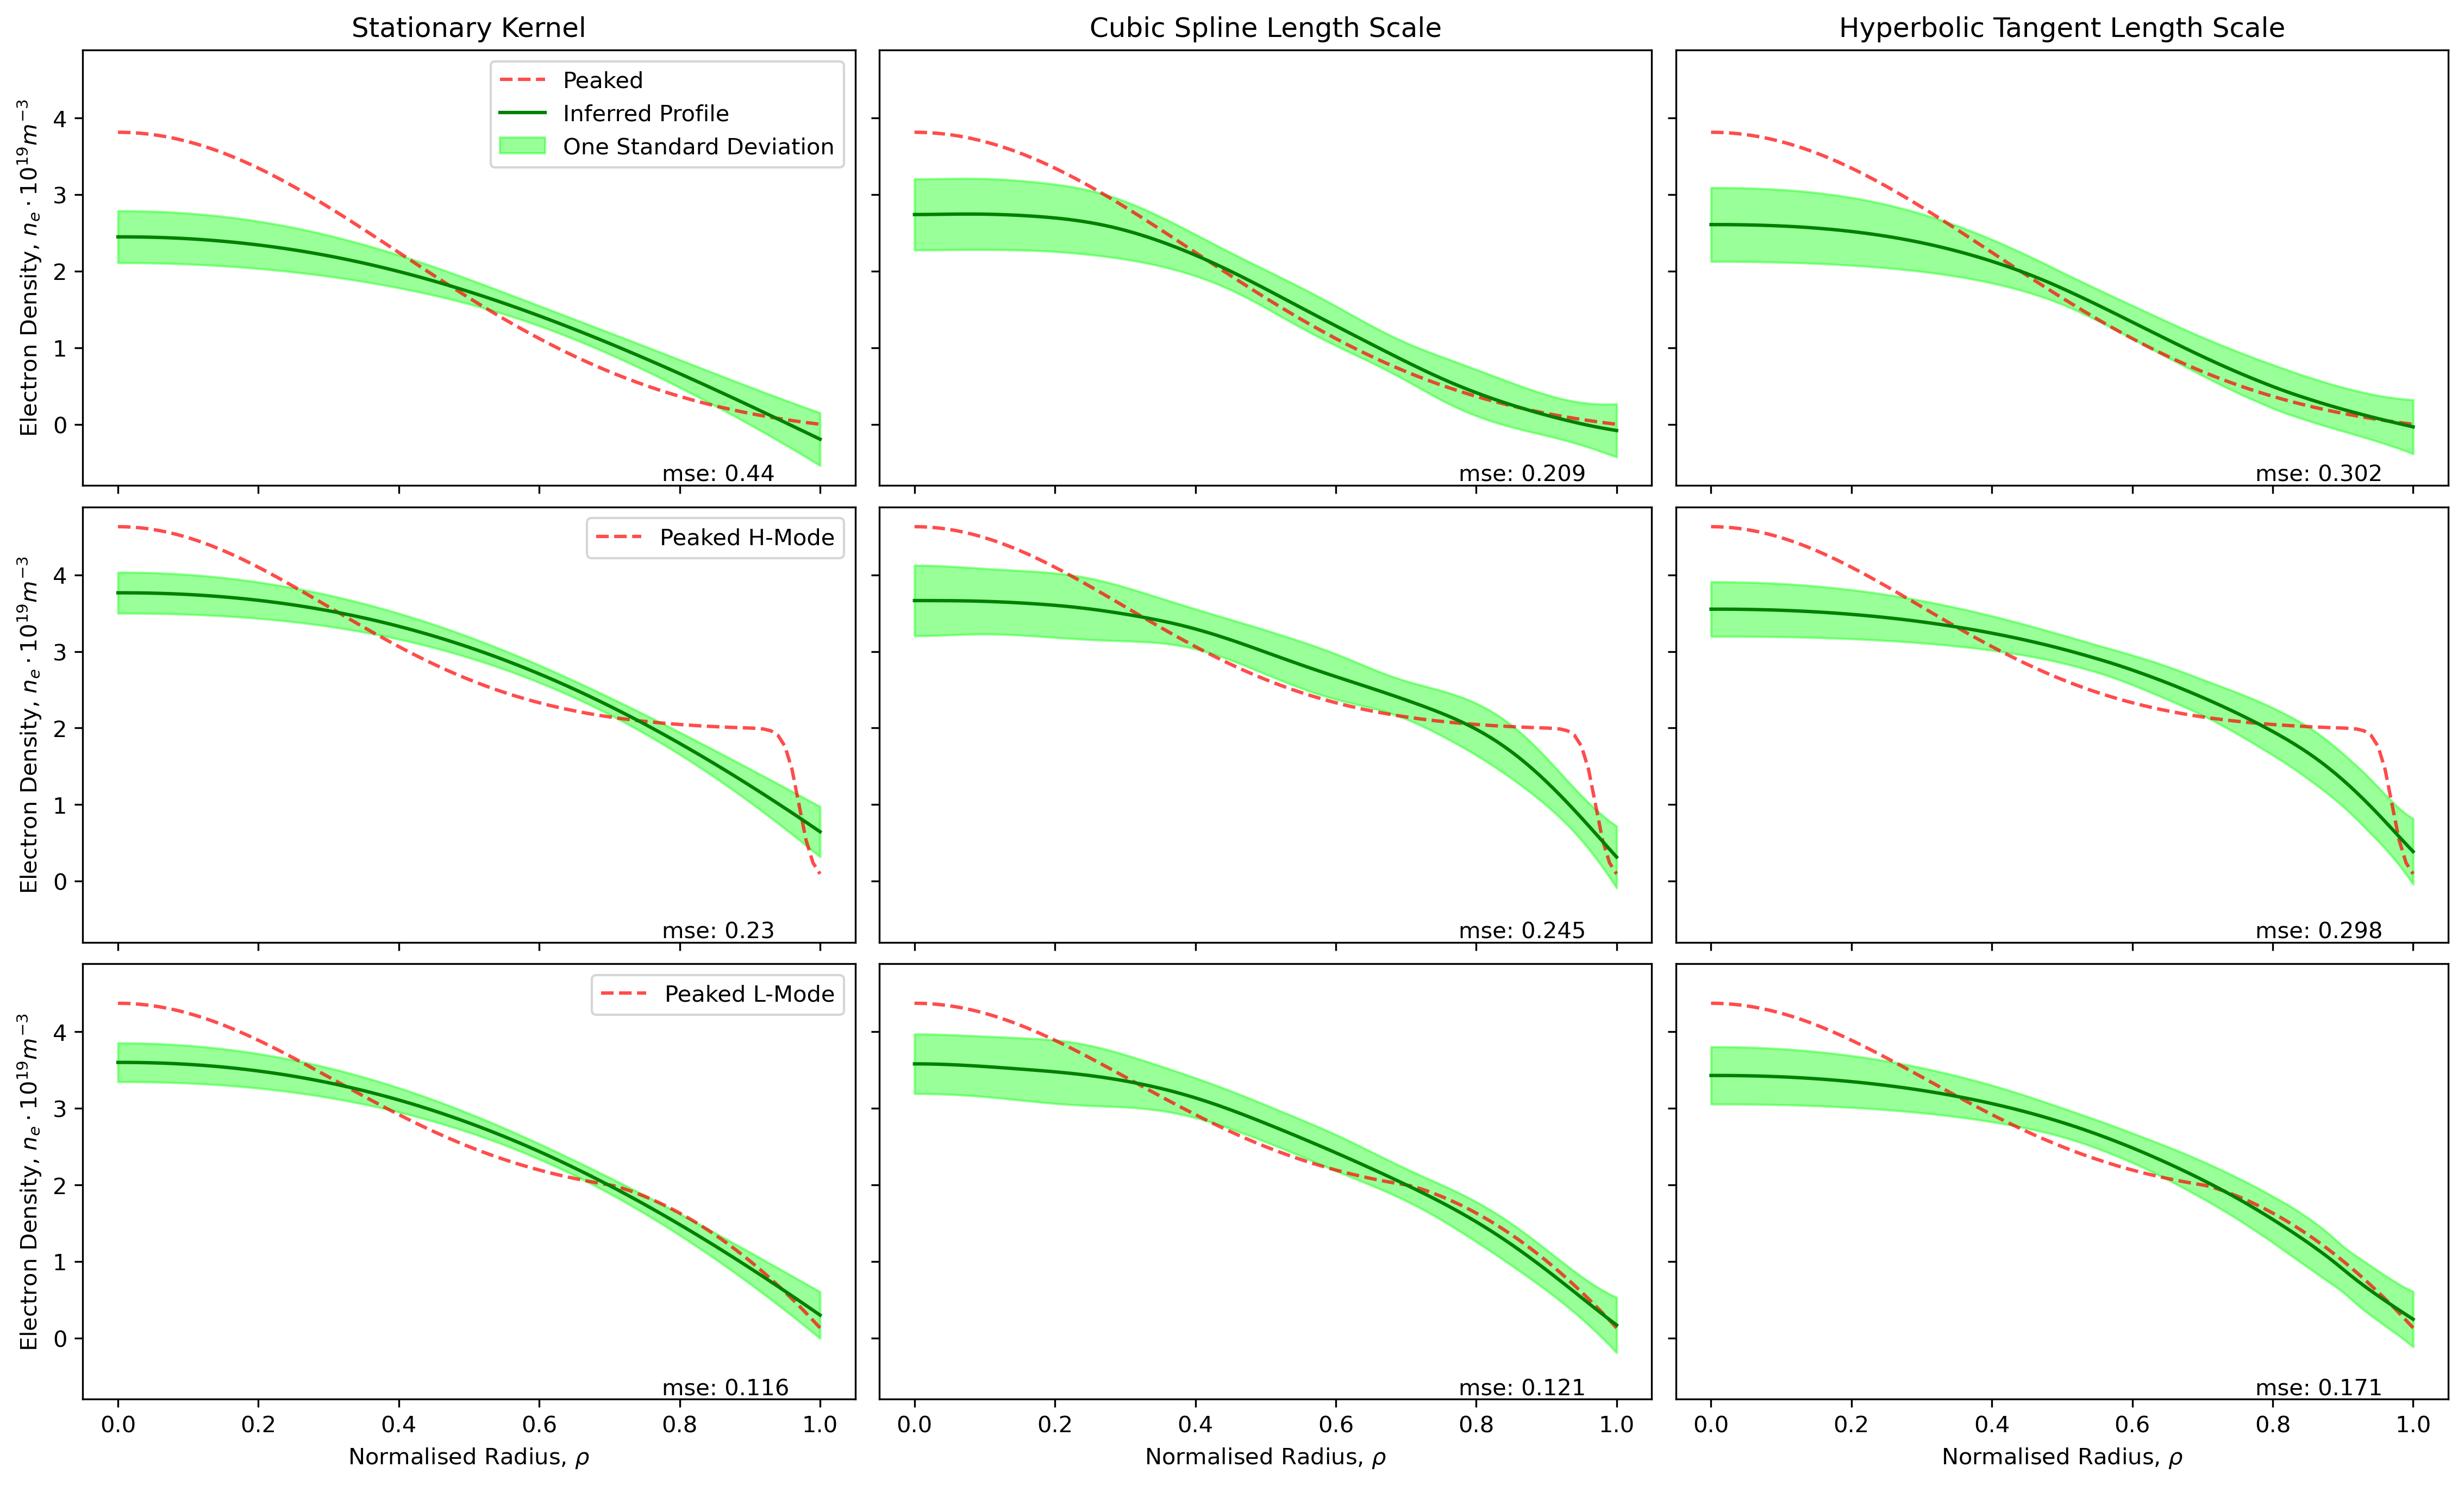
\includegraphics[width=500pt, angle=90]{images/Final/FB6000compute_noMAP_p_burn1000_thin10.png}
    \caption{Electron density inference based on the full Bayesian method for synthetic interferometry data from peaked profiles.}
    \label{fig:fb_inference_p}
\end{figure}

The exact same analysis is executed for real interferometry data from the \gls{west} tokamak. \gls{west} operates in L mode and figure \ref{fig:interf_nice} shows a \gls{nice} inference for a typical set of interferometry data and magnetic flux surfaces. The inferrences from the hyperparameter \gls{map} method are shown in figure \ref{fig:map_real}. 

\begin{figure}[ht]
    \centering
    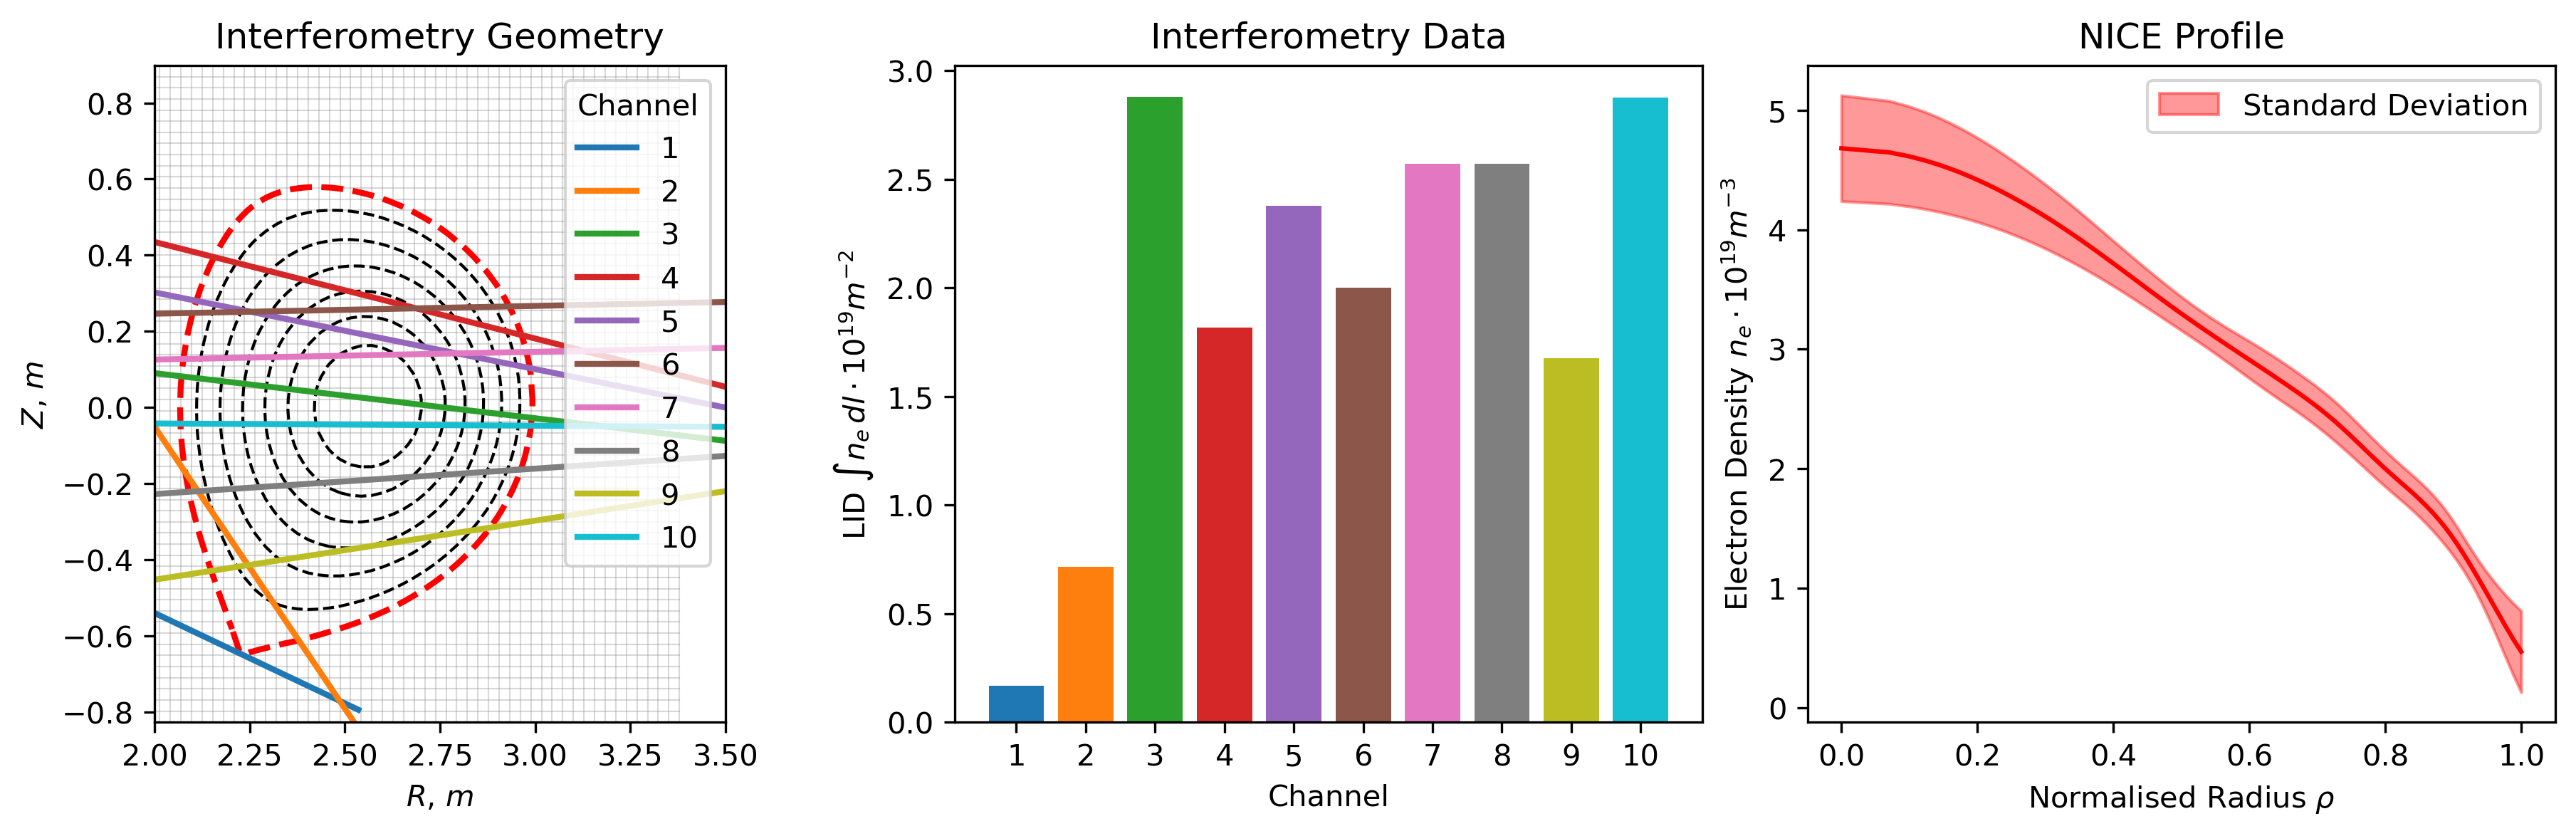
\includegraphics[width=500pt]{images/Final/interferometry_nice.png}
    \caption{A typical set of magnetic flux surfaces and interferometry data from the WEST tokamak. The electron desnity profile inferred by the NICE algorithem.}
    \label{fig:interf_nice}
\end{figure}

\begin{figure}[ht]
    \centering
    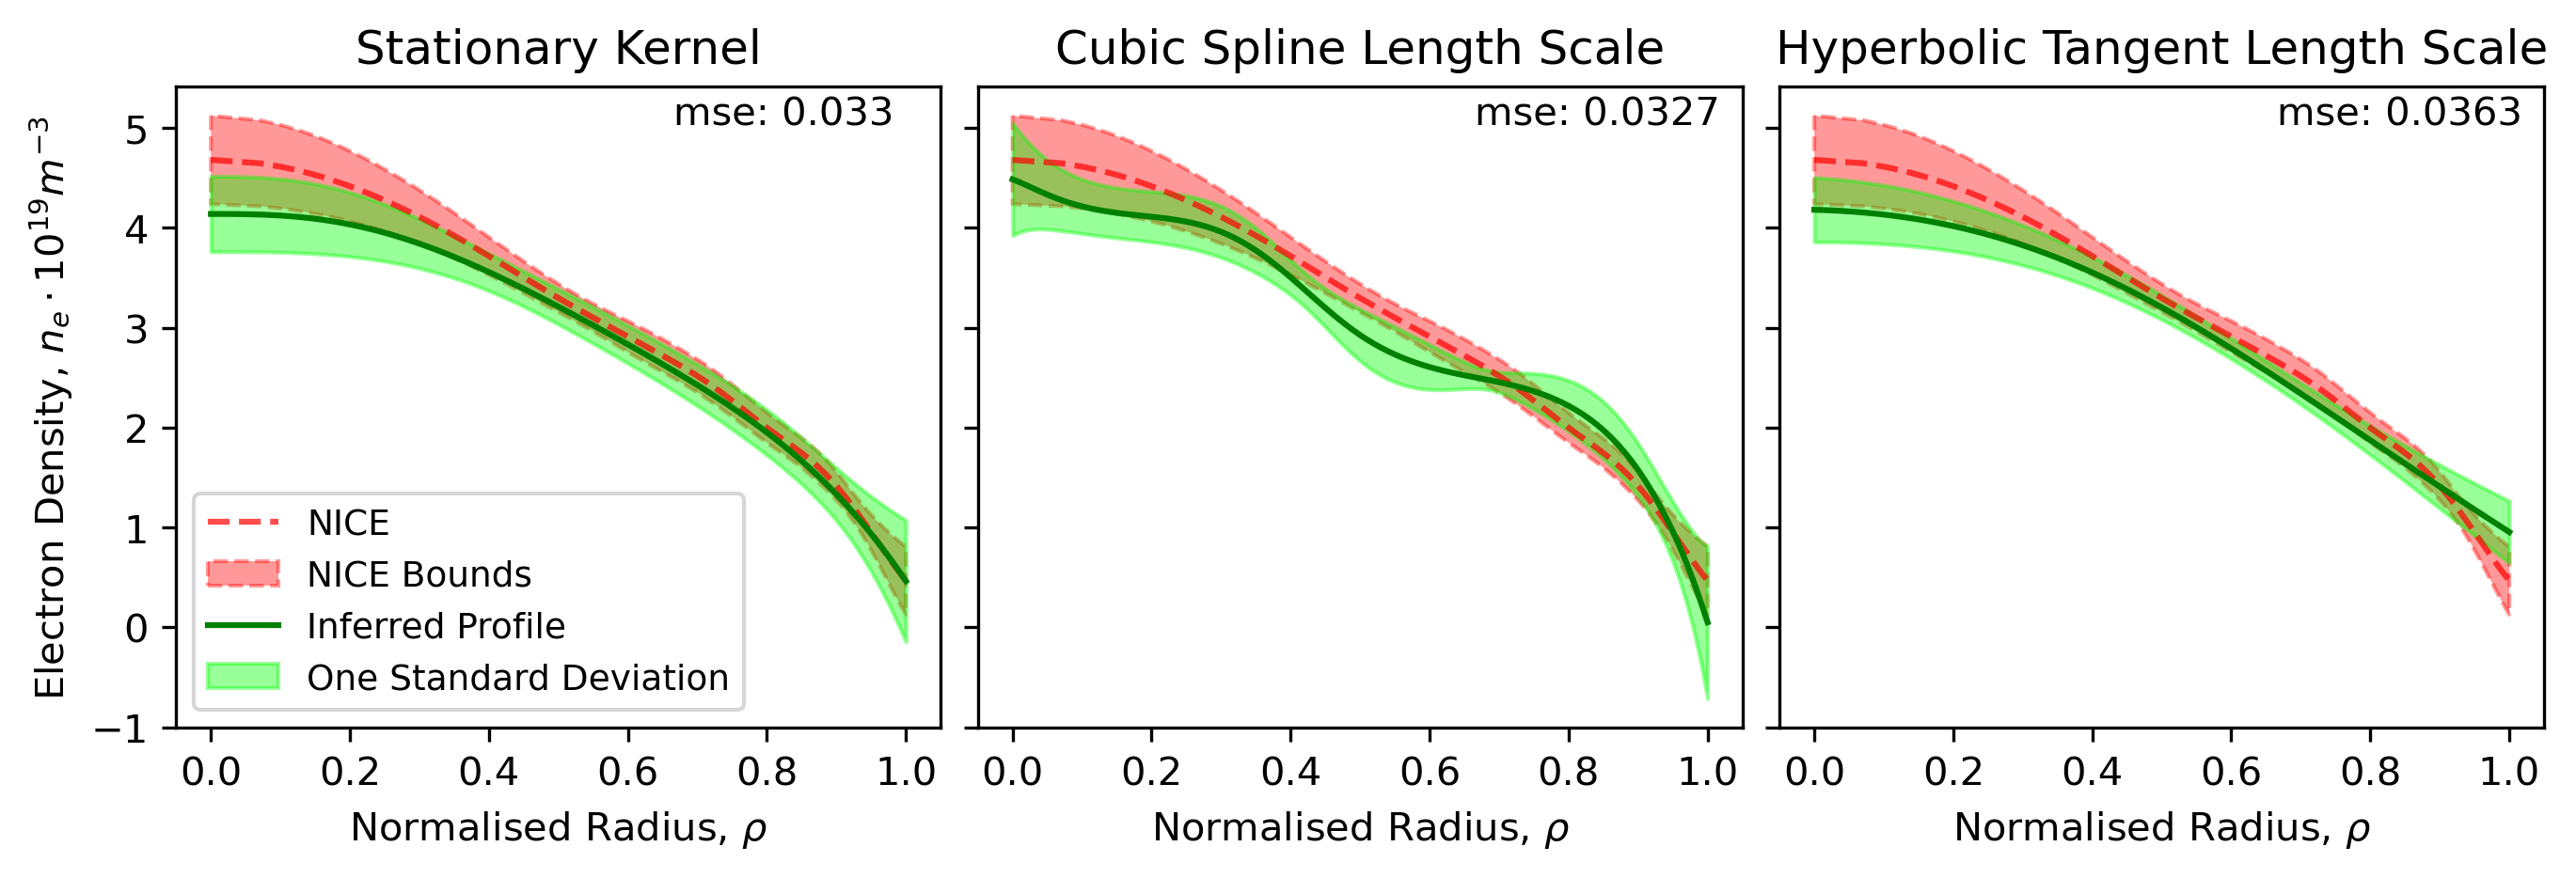
\includegraphics[width=\textwidth]{images/Final/NICE_real_map_likep.png}
    \caption{Electron density inference using the hyperparameter MAP method on real interferometry data from the WEST tokamak. The mean square error is shown as `mse'.}
    \label{fig:map_real}
\end{figure}

% \begin{figure}[ht]
%     \centering
%     \includegraphics[width=\textwidth]{images/Final/NICE_real_fb_likep.png}
%     \caption{Electron density inference using the full Bayesian method on real interferometry data from the WEST tokamak. The mean square error is shown as `mse'.}
%     \label{fig:map_real}
% \end{figure}




% \begin{table}
% \centering
% \begin{tabular}{|c|c|c|}
%     \hline
%     \textbf{Hyperparameter} & \textbf{Lower Bound} & \textbf{Upper Bound} \\
%     \hline
%     Amplitude & 0 & 100 \\
%     Length Scale & 0 & 3 \\
%     \hline
%     \textbf{Hyperbolic Tangent} & &\\
%     Transition Center & 0 & 1 \\
%     Transition Width & 0.01 & 0.5 \\
%     \hline
%     \textbf{Cubic Spline} & & \\
%     5 Knots Evenly Spaced in $rho$ & & \\
%     \hline
% \end{tabular}
% \caption{}
% \label{tbl:prior}
% \end{table}

%methodology

% Explain the details of the how the theory is implimented, what processing power is required, I used python jupyter notebooks numpy, scipy and pytorch. Explain the key parts of the code in order to compute the kernels, marginal likelyhood and inference. What test were done in order to try and improve the inference. 

% \begin{itemize}
%     \item What format was the data in when it came from west and how did I import it into python
%     \item A bit about the diffent forms the data comes in on the west imas database and which one was chosen. 
%     \item How can the accuracy of the forward model be tested and how should this effect the experimental error.
%     \item How does one select an experimental error, is it important for the inference? 
%     \item What is the non positive definite matrix error, how can it be avoided, what are the implications of this
%     \item How I used meshgrid to compute the kernel in a fast way
%     \item what are the different methods used for finding the minimum of the marginal likelyhood, scipy minimize, pytorch, grid search. How do they work. 
%     \item What distributions did I use to randomly initialize the kernel parameters. Why did I randomly initialise them?
%     \item Why I coded everything with pytorch tensors
%     \item How I optimised the learning rate
%     \item Attempts to use noise
%     \item How did I try and improve the inference.
%     \item summarise the chapter and lead into the results. 
    
% \end{itemize}


% \begin{itemize}
%     \item Make the case as why a 0 mean prior is not always a good Idea, since the marginal likelyhood is not perfect and inferences favour the lower side of NICE, likely due to the 0 prior as when amp is increased the inference will move to NICE but not beyond it. Including prior knowledge when available is always advised.
    
%     \item Make the case that if I set NICE as the true ground truth and create synthetic data then I get the NICE profile from lowering marginal likelyhood. This shows that everything is set up correctly.
    
%     \item Show I am getting a local minimum of the marginal likelihood which is nice like and a lower minimum which is parabolic. This could be a result of the marginal likelihood not being a perfect loss function for problems with little data. This seems to be true for SciPy, PyTorch, static and non-static.
%     \item Talk about the discovered more defined ridge, ask for access to log book to see if this is during a H-mode shot. Explain why it might be physically significant but a full monte carlo bayesian should be carried out to verify this. 
%     \item Show the static grid search

%     \item Results not yet curated
%         \subitem Bayesian inference using monte carlo methods
%         \subitem One size fits all kernel for real time. 
%     \item summarise the chapter and lead into conclusions
% \end{itemize}




%Figure \ref{fig:trace6000} shows a trace plot for the static lengthscale samples from a 6000 sample chain. 
% \begin{figure}[ht]
%     \centering
%     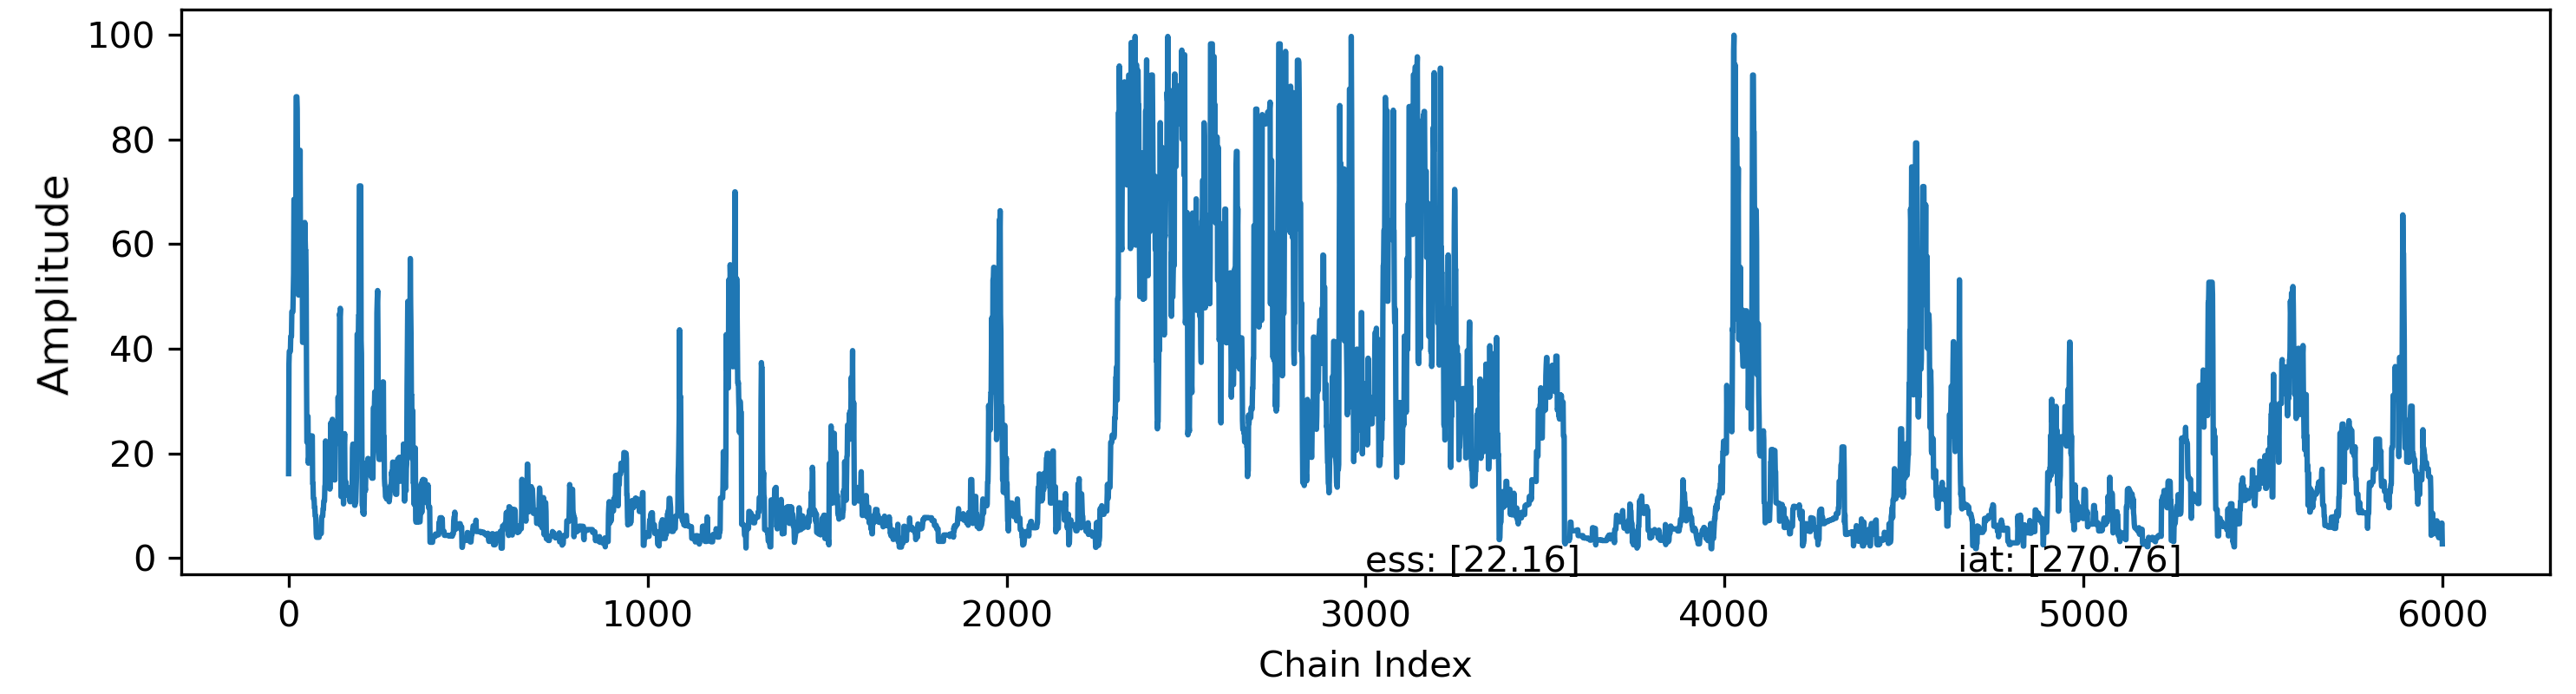
\includegraphics[width=\textwidth]{images/Final/Trace.png}
%     \caption{A trace plot showing the 6000 amplitude samples taken by an emcee chain. The integrated autocorrelation time and effective sample size is shown as `iat' and `ess', respectivly.}
%     \label{fig:trace6000}
% \end{figure}